\documentclass[11pt]{article}
\usepackage{graphicx}
\usepackage{amsmath}
\usepackage{amssymb}
\usepackage{float}
\usepackage{commath}
\usepackage{siunitx}
\sisetup{detect-all}
\usepackage[a4paper,margin=20mm]{geometry}
\begin{document}
\title{\textbf{UCL Mechanical Engineering 2020/2021}\\MECH0013 Coursework 2}
\maketitle
\textit{Model Details:}

Same parameters specified in \textit{Methodology} are used. The single change is that the beam is reduced in length to \SI{0.8}{\meter}.

\textit{Analysis:}
The critical force for mode 1 can be calculated using the following equation
\begin{gather}
    L_e = 1 \hspace{1cm} l = \SI{0.8}{\meter}\\
    S_{cr} = \frac{1^2 \cdot \pi^2 \cdot\left(207\cdot10^9\right)\cdot\left(1.125\cdot 10^{-7}\right)}{(1\cdot 0.8)^2} = \SI{369122.5195}{\newton}
\end{gather}
Under the specifications provided above, the buckling of the beam was simulated. The total deformation pattern of the beam is provided in Figure (\ref{q3ss}) below:
\begin{figure}[H]
    \centering
    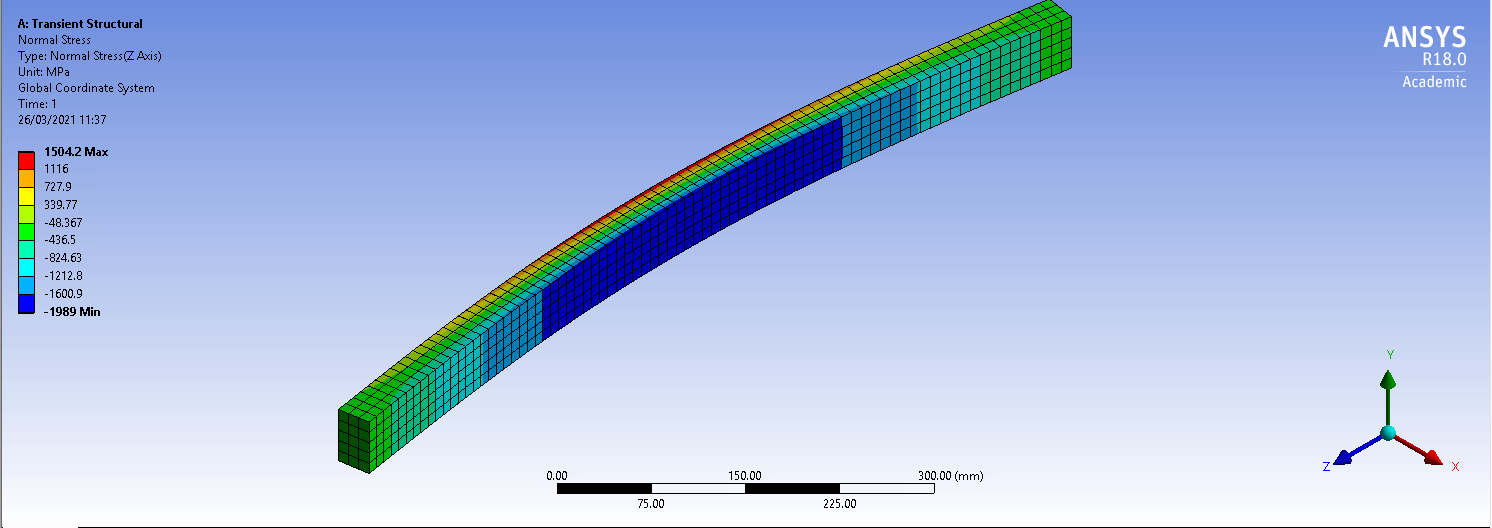
\includegraphics[width=0.6\textwidth]{q3normalstress1.png}
    \caption{Normal stresses along the beam in buckling}
    \label{q3ss}
\end{figure}
The Force Reaction tool on ANSYS was utilized to obtain the temporal axial force along the beam. The results were plotted against time on MATLAB and presented on Figure (\ref{q3axial}) below. The maximum analytical load, calculated above, was also included as a constant value.
\begin{figure}[H]
    \centering
    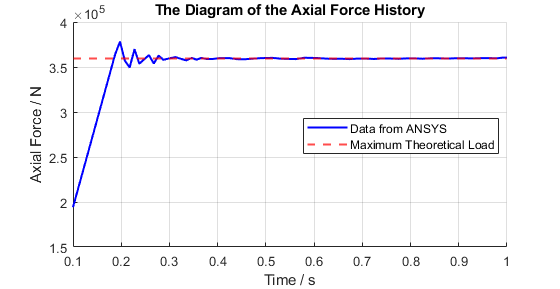
\includegraphics[width=0.6\textwidth]{q3axial.png}
    \caption{Axial force history diagram of the shortened beam.}
    \label{q3axial}
\end{figure}
In Figure (\ref{q3stress}) below, the maximum stress values from both the simulation and the analytical results were plotted against the deflection along the beam.
\begin{figure}[H]
    \centering
    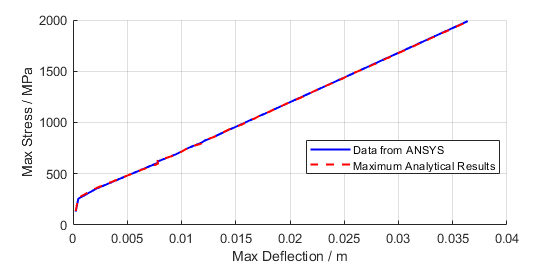
\includegraphics[width=0.6\textwidth]{q3def.png}
    \caption{The maximum stress as a function of maximum deflection for the shortened beam.}
    \label{q3stress}
\end{figure}
\textit{Discussion:}

The data from our simulation gives us stress data which is aligned with our analysis. We see that the maximum theoretical load is reached at a later time than with a beam of length \SI{1}{\meter}. This can be attributed to the fact that more force is required to buckle the beam. We see a similarity with there being an oscillatory overshoot before a stabilisation in the axial force. This may be due to application restrictions, such as mesh sizing and transient simulation options. 

The maximum stress as a function of the deformation followed closely to our analytical expectation. Both plots have a linear increase. This shows us that ANSYS can reflect the deflection of a beam buckling under compressive loads accurately. 

\textit{Model Details:}

The standard model details, mentioned previously were used with some changes. The support configurations were changed to a fixed-fixed arrangement. One end was fixed using the 'Fixed support.' At the other end, 'Remote displacement' is used and rotation is fixed. A small transient displacement of 5mm is applied in the z-direction to facilitate compression. 

\textit{Analysis:}

The critical force can be calculated using the following equation:
\begin{gather}
    L_e = 0.5 \hspace{1cm} l = \SI{1}{\meter}\\
    S_{cr} = \frac{1^2 \cdot \pi^2 \cdot\left(207\cdot10^9\right)\cdot\left(1.125\cdot 10^{-7}\right)}{(0.5\cdot 1)^2} = \SI{919353.65}{\newton}
\end{gather}
Under the specifications provided above, the buckling of the beam was simulated. The total deformation pattern of the beam is provided in Figure (\ref{q5ss}) below:
\begin{figure}[H]
    \centering
    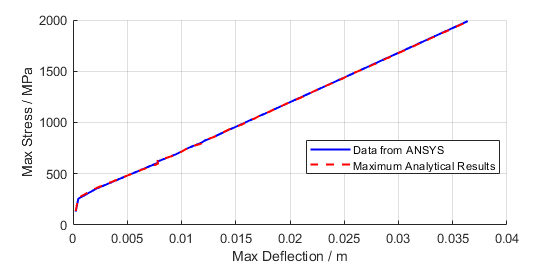
\includegraphics[width=0.6\textwidth]{q3def.png}
    \caption{}
    \label{q5ss}
\end{figure}
The Force Reaction tool on ANSYS was utilized to obtain the temporal axial force along the beam. The results were plotted against time on MATLAB and presented on Figure (\ref{q5axial}) below. The maximum analytical load, calculated above, was also included as a constant value.
\begin{figure}[H]
    \centering
    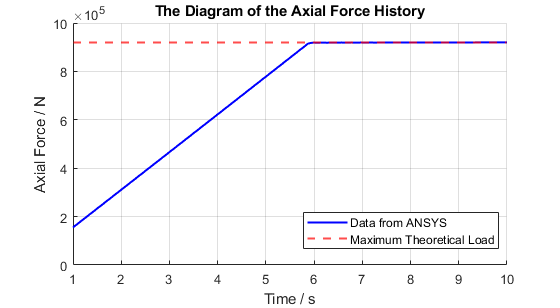
\includegraphics[width=0.6\textwidth]{q5axial.png}
    \caption{Axial force history diagram of the fixed-fixed beam.}
    \label{q5axial}
\end{figure}
In Figure (\ref{q3stress}) below, the maximum stress values from both the simulation and the analytical results were plotted against the deflection along the beam.
\begin{figure}[H]
    \centering
    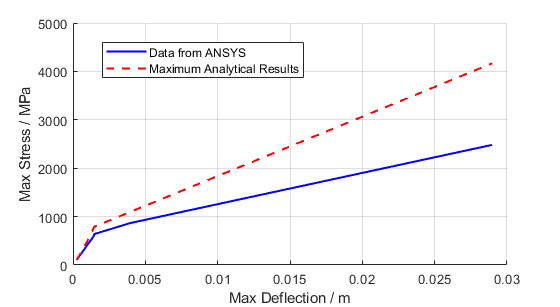
\includegraphics[width=0.6\textwidth]{q5def.png}
    \caption{The maximum stress as a function of maximum deflection for the fixed-fixed beam.}
    \label{q5stress}
\end{figure}

\textit{Discussion:}

The determined critical load and our simulated load closely match. As seen in Figure (\ref{q5axial}), the axial force line behaves like an asymptotic curve, with no oscillatory overshoot. We see an initial linear increase until the maximum theoretical load is reached. Afterwards there is a very slight increase in axial load due to further increasing compression, however this is much smaller as the buckling has been initiated.

The maximum stresses in this beam, shown in Figure (\ref{q5stress}), both analytical and experimental data, increased with increasing deflection, however the results did not match closely. We see that our data from ANSYS shows a much lower stress for given deflection than our theoretical result. This error increases with deflection. Looking at our ANSYS simulation, we found that the maximum stresses were occurring at both fixed ends, instead of the middle of the beam. Our theoretical analysis calculates the stress based on the maximum deflection in buckling, which cannot be applied to the undeflected fixed ends. However, it may still be accurately representing the stress in the middle of the beam (where deflection is maximum)
\end{document}